\begin{center}
    % Gain
    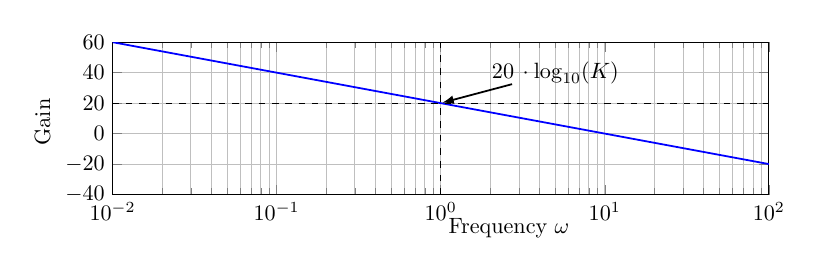
\begin{tikzpicture}
        [
            scale = 0.8,
            >=latex
        ]
        \begin{axis}
            [
                width=12cm,
                height=4cm,
                xmode=log,
                xmin=0.01, xmax=100, ymin=-40, ymax=60,
                x label style={anchor=west},
                xlabel=Frequency $\omega$,
                y label style={anchor=south},
                ylabel=Gain $\deci \bel$,
                xmajorgrids=true,
                xminorgrids=true,
                ymajorgrids=true
            ]

            % Plot
            \addplot[thick, color=blue, domain=0.01:100]{-20*log10(x)+20};
            
            % guide lines
            \addplot[dashed, color=black, domain=0.01:100]{20}; 
            \addplot [dashed, color=black] coordinates {(1, -40) (1, 60)};
           
            % Node / Label
            % \node (p) at (0.01, 20) {$20 \, \deci \bel \cdot \log_{10}(K)$};
            \node[inner sep=0pt] (p) at (1, 20) {};
            \node[inner sep=0pt] (q) at (5, 40) {$20 \, \deci \bel \cdot \log_{10}(K)$};

            \draw[->, thick, color=black] (q) -- (p);


        \end{axis}
        
    \end{tikzpicture}


    % Phase
    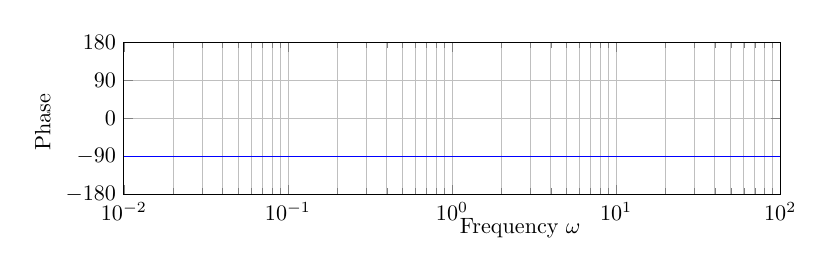
\begin{tikzpicture}
        [
            scale = 0.8,
            >=latex
        ]
        \begin{axis}
            [
                width=12cm,
                height=4cm,
                xmode=log,
                xmin=0.01, xmax=100, ymin=-180, ymax=180,
                x label style={anchor=west},
                xlabel=Frequency $\omega$,
                y label style={anchor=south},
                ylabel=Phase $\degree$,
                ytick={-180, -90, 0, 90, 180},
                % yticklabels={-180, -90, 0, 90, 180},
                xmajorgrids=true,
                xminorgrids=true,
                ymajorgrids=true
            ]
            
            % Phase
            \addplot[thick, color=blue, domain=0.01:100]{-90};
                
        \end{axis}
            
    \end{tikzpicture}
\end{center}